\section{Objectives}
\label{sec-objectives}
The main goal in this study is to detect seizures from the dataset CHB-MIT. To fulfil the objective an architecture has been created working within a pipeline of events. Starting by finding the best data analysis and processing method before feeding it to the deep learning algorithms. There are many sub-objectives to be completed to obtain good results from this architecture and also, it’s modular for further expansion and studies. The main strategy of the scripts execute in sequence (Fig. 1)
\\

Within the objective of data classification, another objective to find the most precise architecture is defined to obtain results with the most accuracy possible. In order to fulfil these objectives a set of sub objectives have been defined. The following points summarize the set of subobjectives:
\\
\begin{enumerate}

\item Raw data must be readable, as the data base CHB-MIT is in European Data Format (EDF), a standard file format designed for exchange and storage of medical time series, all files in the dataset are in edf format. A script has been programmed to save edf files into parquet format. Parquet is needed to be able to handle data more easily, as well as improving compatibility with other related work scripts from the CVC.
\item Setting different functions to filter data, making sure data fits certain constraints to obtain better results when training the model. This makes the script modular to obtain data from the dataset CHB-MIT.
\item Label raw data, to have a ground truth from the provided summary files in the dataset.  This part is essential to understand if the model works as expected.
\item Functions create constraints on the dimensionality of the data to fit the input of the model as well as filtering data from the dataset. This functions filter in bandwidth of the data, and excluding files from the dataset where data is not well recorded.
\item Each model needs to be configured to accept the dimensionality of the data fed to it. All data must be in two files of numpy arrays and all input must have the same dimensions. This will make sure all files are read the same way, and the model will train with uniform data.
\item Work different models to choose what models give better answers form input data. The CVC provides different models adapted to related work. These models have different inputs and are initialized in different ways. All models must be initialized and executed the same way, to make it easier to train and test more than one model, to obtain different answers.
\item After all the models results, an overview is done to understand the results and conclude the best way to treat this database, for further investigation.
    
\end{enumerate}
\begin{figure}[H]
    \caption{Scheme of data processing }
    \centering
    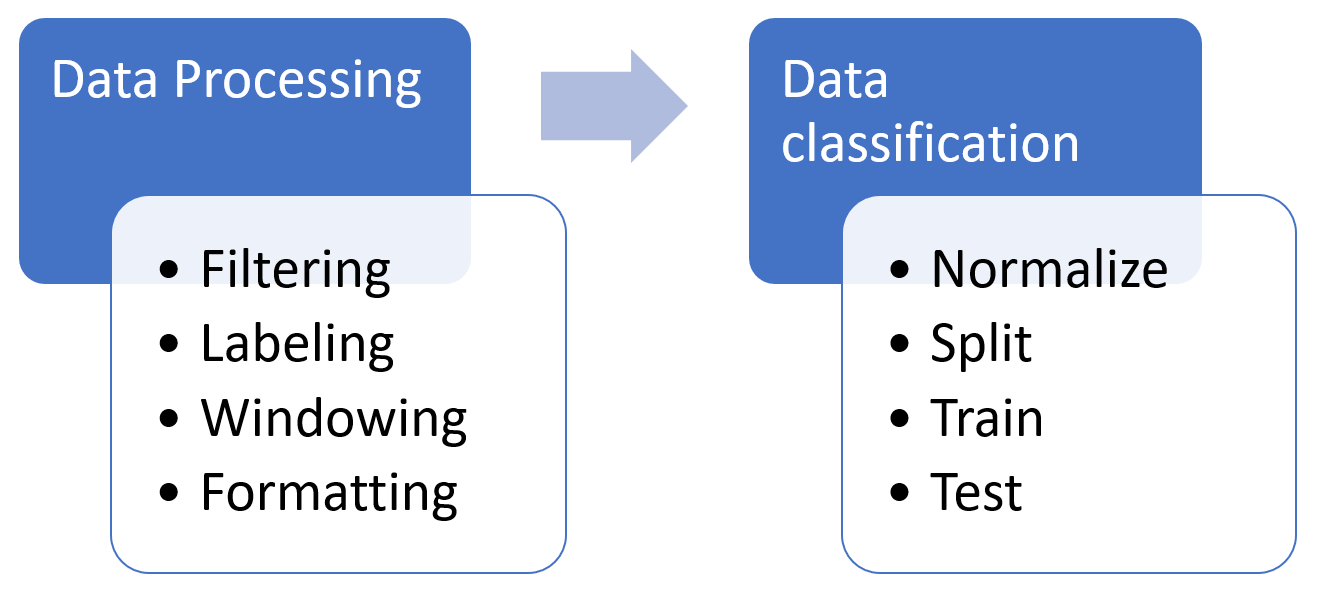
\includegraphics[width=0.5\textwidth]{img/pipeline.png}
\end{figure}
\leavevmode\\